\section{Diffusion du véhicule électrique}

	\subsection{Différents modèles de diffusion}
	
		Le modèle de diffusion de Bass sert avant tout à prévoir l'évolution de l'adoption d'un nouveau produit dans une population donnée. Ainsi, il décrit l'intégration des innovations technologiques dans la population. Notre objectif est ici de déterminer le nombre de véhicules électriques en circulation en 2025. Étant donné qu'il existe peu d'études sur le sujet, il est judicieux d'adopter un modèle type Bass pour mesurer l'évolution de ce marché dans les prochaines années.
		
		
		Selon la théorie de Bass, on peut classer les utilisateurs en grandes classes : les innovateurs, les \emph{early adopters}, les \emph{early majority}, les \emph{late majority} et les retardataires. Cette classification, illustrée par la figure \vref{fig.BassUtilisateurs}, se fait par l'intermédiaire de deux facteurs essentiels: l'hétérogénéité des agents sociaux (aversion au risque, milieu social), et la capacité intellectuelle de l'individu.
		
		\begin{figure}[!h]
			\centering
			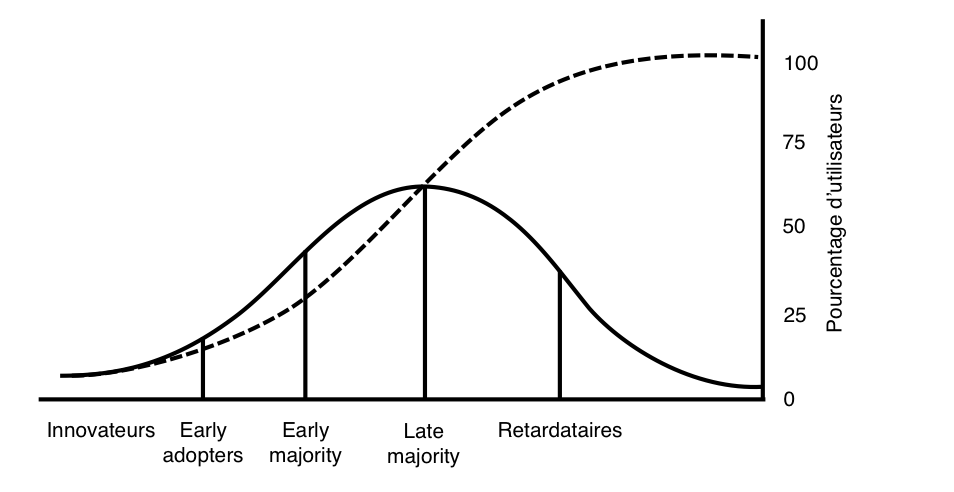
\includegraphics{fig/BassUtilisateurs.eps}
			\caption{Évolution du nombre d'utilisateurs d'une innovation technologique selon le modèle théorique de Bass. \label{fig.BassUtilisateurs}}
		\end{figure}
		
		Les modèles de diffusion peuvent être résumés dans une seule équation différentielle: 
		\[
			\dfrac{\D N(t)}{\D t} = g(t)(m-N(t))
		\]
		où $N(t)$ est le nombre cumulé d'individus ayant adopté la technologie à la date $t$, $m$ est le seuil maximal du nombre d'acheteurs potentiels, c'est-à-dire la taille du marché, et $g(t)$ le \emph{coefficient de diffusion}.
		
		En fonction de la valeur du coefficient de diffusion $g(t)$, on trouve 3 modèles essentiels :
		\begin{enumerate}
			\item modèle des influences externes: $g(t) = p = \text{cste}$.
			Dans ce modèle, le paramètre $p$ peut être interprété comme l'ensemble des facteurs extérieurs qui agissent sur la prise de décision du consommateur (pouvoir des médias et des réseaux sociaux, par exemple);
			\item modèle des influences internes: $g(t) = q N(t)$ où $q$ est le \emph{coefficient d'imitation}. Dans ce modèle, le paramètre $q$ représente l'interaction entre les acheteurs potentiels et ceux qui ont déjà adopté la technologie, car pour un futur acheteur l'avis des autres consommateurs est primordial;
			\item modèle de Bass : $g(t) = p + q \frac{N(t)}{m}$. C'est un mélange des deux modèles précédents. Ainsi, sur un intervalle de temps $\Delta t$, le nombre d'individus qui adoptent la technologie est régi par deux phénomènes: 
			\begin{itemize}
				\item contagion, fonction du nombre d'individus ayant déjà adopté l'innovation (terme $q N(t)(m - N(t))$);
				\item saturation du fait de la présence du palier $m$.
			\end{itemize}
			La solution à ce problème est:
				\[
					N(t) = \dfrac{m - \dfrac{p (m - N_0)}{p + q \frac{N_0}{m}} \mathrm{e}^{-(p+q)t}}{1 - \dfrac{\frac{q}{m} (m - N_0)}{p + q \frac{N_0}{m}} \mathrm{e}^{-(p+q)t}}
				\]
			avec $N_0 = N(t = 0)$.
		\end{enumerate}
		
		Mais tous les modèles précédents supposaient l'existence d'une taille de marché $m$ constante. Cependant, en général, ce n'est pas le cas: on peut considérer l'arrivée de nouveaux conducteurs, les voitures qui parviennent en fin de vie... C'est pour cette raison que l'on adoptera dans notre approche le modèle de Sharif et Ramannathan avec une taille de marché dépendante du temps : $m(t) = m_0 \mathrm{e}^{gt}$.
		
		
		La résolution mathématique de ce problème se présente sous cette forme :
		\begin{gather*}
			N(t) = m_0 \mathrm{e}^{gt} \dfrac{\dfrac{\Phi_1 - \Phi_2}{2} - \Phi_3 \dfrac{\Phi_1 + \Phi_2}{2} \mathrm{e}^{-\Phi_1 t}}{q + q \Phi_3 \mathrm{e}^{-\Phi_1 t}} \quad \text{où} \\
			\Phi_1 = \sqrt{(g+p-q)^2 + 4pq} \qquad \Phi_2 = g + p - q \qquad \Phi_3 = \dfrac{\frac{\Phi_1 - \Phi_2}{2} - q \frac{N_0}{m_0}}{\frac{\Phi_1 + \Phi_2}{2} + q \frac{N_0}{m_0}}, \; (0 < N_0 \leqslant m_0).
		\end{gather*}


	\subsection{Utilisation des modèles de diffusion pour le marché du véhicule électrique}

		L'implémentation des modèles précédents pour l'étude du marché des véhicules électriques nécessite la détermination des paramètres $p$, $q$, $N_0$ et $m$ (ou $m_0$ et $g$).

		Pour ce faire, nous utilisons comme données d'entrée le tableau \vref{tab.immatriculeConception} qui est issu de chiffres préfectoraux:
		
	
			
		\begin{table}[!h]
			\centering
			{\footnotesize
			\csvautotabular{fig/tableau1.csv}}
			\caption{Nombres mensuels d'immatriculations de véhicules électriques entre janvier 2011 et mars 2015. \label{tab.immatriculeConception}}
		\end{table}

		Nous nous intéressons dans un premier temps au modèle classique de Bass, dans lequel le paramètre $m$ ne dépend pas du temps.

		La grandeur $N_0$ se lit directement sur la première ligne du tableau de données: en effet, les immatriculations de voitures électriques sont extrêmement faibles avant janvier 2011 et le volume de ces véhicules peut être considéré comme négligeable. Nous prenons donc $N_0 = 100$.

		Les autres paramètres s'obtiennent par utilisation de la méthode OLS qui nous a paru la plus appropriée et la plus fidèle. Le tracé de $X(t) = N(t) - N(t-1)$ en fonction de $N(t-1)$ donne la courbe de la figure \vref{fig.courbeXt}.
		
		\begin{figure}[!h]
			\centering
			\begin{tikzpicture}
				\begin{axis}[ 
				/pgf/number format/.cd,
				use comma,
				1000 sep={ },
				height = 8cm,
				width = 15cm,
				axis x line = bottom,
				axis y line = left
 				]
				\addplot[mark = +, draw = blue, smooth] file{fig/courbeXt.txt};
				\addplot[color = red, domain = 0:30000] {-4.55*10^(-7)*x^2+0.0414*x+238.79};
				\end{axis}
			\end{tikzpicture}
			\caption{Tracé de $X(t)$ en fonction de $N(t-1)$.\label{fig.courbeXt}}
		\end{figure}
		
		Une courbe polynomiale de second degré $X(t) = \alpha_1 + \alpha_2 N(t-1) + \alpha_3 N(t-1)^2$ s'ajuste au graphique obtenu avec les valeurs suivantes (coefficient de corrélation $R^2 = \num{0.49}$):
		\begin{align*}
			\alpha_1 &= \num{238.79}\\
			\alpha_2 &= \num{0.04141}\\
			\alpha_3 &= \num{-4.55e-7}
		\end{align*}

		On obtient les paramètres suivants :
		\begin{align*}
			p &= \dfrac{-\alpha_2 + \sqrt{\alpha_2^2 - 4 \alpha_1 \alpha_3}}{2} = \num{0.0024743185}\\
			q &= \dfrac{\alpha_2 + \sqrt{\alpha_2^2 - 4 \alpha_1 \alpha_3}}{2} = \num{0.0438843185}\\
			m &= \dfrac{-\alpha_2 - \sqrt{\alpha_2^2 - 4 \alpha_1 \alpha_3}}{2 \alpha_3} = \num{96507}
		\end{align*}

		L'ordre de grandeur de $m$ parait cohérent, le nombre de véhicules électriques roulant en 2014 étant d'environ \num{30000}. Ceci nous permet d'obtenir le profil de diffusion de la figure \vref{fig.courbeBass1}, dont la limite est égale à $m = \num{96507}$.

		\begin{figure}[!h]
			\centering
				\begin{tikzpicture}
					\begin{axis}[
					height = 8cm,
					width = 15cm,
					axis x line = bottom,
					axis y line = left,
					xlabel = mois,
					ylabel = nombre d'utilisateurs cumulés
					]
					\addplot[mark = none, draw = blue, smooth] file{fig/courbeBass.txt};
					\end{axis} 
				\end{tikzpicture}
			\caption{Profil de diffusion selon le modèle de Bass.\label{fig.courbeBass1}}
		\end{figure}

		Ce modèle semble avoir une durée de validité assez faible, puisque le palier $X = m$ est obtenu avant 2025. Essayons donc d'implémenter le modèle plus réaliste de Sharif et Ramannathan, dans lequel la capacité globale du marché $m$ dépend du temps, selon une loi exponentielle: $m(t) = m_0 \mathrm{e}^{gt}$.
		Nous reprenons les mêmes coefficients d'innovation $p$ et d'imitation $q$ que précédemment. Il est également logique d'adopter $m_0 = \num{96507}$ puisque $m(t = 0) = m_0$.
		Reste enfin à trouver une valeur pour le coefficient $g$. N'ayant aucune méthode à notre disposition pour le déterminer, nous adoptons $g = 0,035$ \footnote{Valeur utilisée dans une étude sur la diffusion de l'accès à Internet, au sein de la population française (A. Kijek, T. Kijek, \textit{Operations research and decisions}, \textbf{2010}, 3-4, \textit{53-68}).}.
		Le graphe obtenu présenté en figure \vref{fig.SharifRaman}.
		
		\begin{figure}[!h]
			\centering
			\begin{tikzpicture}
				\begin{axis}[
				height = 8cm,
				width = 15cm,
				axis x line = bottom,
				axis y line = left,
				xlabel = mois,
				ylabel = nombre d'utilisateurs cumulés
				]
				\addplot[mark = none, draw = blue, smooth] file{fig/SharifRaman.txt};
				\end{axis}
			\end{tikzpicture}
			\caption{Profil de diffusion selon le modèle de Sharif et Ramannathan.\label{fig.SharifRaman}}
		\end{figure}
		
	\clearpage
		
	\subsection{Conclusion}
		
		Les résultats obtenus sont insuffisants. Le premier profil montre une saturation trop rapide, le marché étant supposé de taille fixe $m$: le point d'inflexion est atteint à $t^* = -\dfrac{1}{p+q} \log{\frac{p}{q}} = 62 \text{ mois}$.

		En ce qui concerne le deuxième modèle utilisé, le profil obtenu ne correspond pas aux données que nous avions initialement. Le graphe de la figure \vref{fig.diverSharifRam} présente la divergence entre la réalité (courbe en pointillés) et la théorie.
		
		\begin{figure}[!h]
			\centering
			\begin{tikzpicture}
				\begin{axis}[
				height = 8cm,
				width = 15cm,
				axis x line = bottom,
				axis y line = left,
				xlabel = mois,
				ylabel = nombre d'utilisateurs cumulés
				]
				\addplot[mark = none, draw = blue, smooth] file{fig/graphe5.txt};
				\addplot[mark =+, draw = red, only marks] file{fig/graphe4.txt};
				\end{axis}
			\end{tikzpicture}
			\caption{Divergence entre la réalité et la théorie de Sharif et Ramannathan \label{fig.diverSharifRam}}
		\end{figure}
		
		De plus, la taille n'est pas illimitée comme le laisserait supposer l'exponentielle $m(t)$ : en réalité, $m$ augmente par paliers, correspondant par exemple aux innovations technologiques... Le temps caractéristique $\tau$ est de 29 mois, ce qui donnerait un modèle valable jusqu'en 2020 environ.
		
		L'extrapolation du premier profil (figure \vref{fig.extraBass}) jusqu'en janvier 2025 nous permet de supposer un nombre d'utilisateurs de véhicules électriques de $N = \num{163000}$ environ. Nous conservons ce chiffre pour l'étude qui suivra.
		
		\begin{figure}[!h]
			\centering
			\begin{tikzpicture}
				\begin{axis}[
				height = 11cm,
				width = 15cm,
				axis x line = bottom,
				axis y line = left,
				xlabel = mois,
				ylabel = nombre d'utilisateurs cumulés
				]
				\addplot[mark = none, draw = blue, smooth] file{fig/courbeBass.txt};
				\addplot[mark=none, ycomb, color = red] plot coordinates{(169,169*1101-22438)};
				\addplot[color = red, domain = 22438/1101:169]{1101*x -22438};
				\end{axis}
				\end{tikzpicture}
			\caption{Extrapolation à partir du modèle de Bass \label{fig.extraBass}}
		\end{figure}